\documentclass[12pt, a4paper]{article}
\usepackage[margin = 1in, top=1.3in]{geometry}
\usepackage[english]{babel}
\usepackage[utf8]{inputenc}
\usepackage{fancyhdr}
\usepackage{amsmath}
\usepackage{bm}
\usepackage{graphicx}
\usepackage{subcaption}
\usepackage[font=small,labelfont=bf]{caption}
 
\pagestyle{fancy}
\fancyhf{}
\rhead{\small{Shaan Ul Haque(180070053)\\ Samarth Singh (180050090) \\ Niraj Mahajan (180050069)}}
\lhead{CS-663 Assignment-3 : Question 1}
\rfoot{Page 1.\thepage}
 
\begin{document}
\vspace*{-22pt}
\section*{Question 1}
\subsection*{Boat Image}
We used a 5*5 window for the calculation of the structure tensor at any point. The standard deviation($\sigma^2$) used was 1.4. The value of k for cornerness measure was 0.04. While to smoothen the image we used a gaussian filter of  standard deviation equal to 0.65. After all the processing we used non-max suppression to get the final cornerness measure. Results are shown below. 

\begin{figure}[h!]
  \centering
    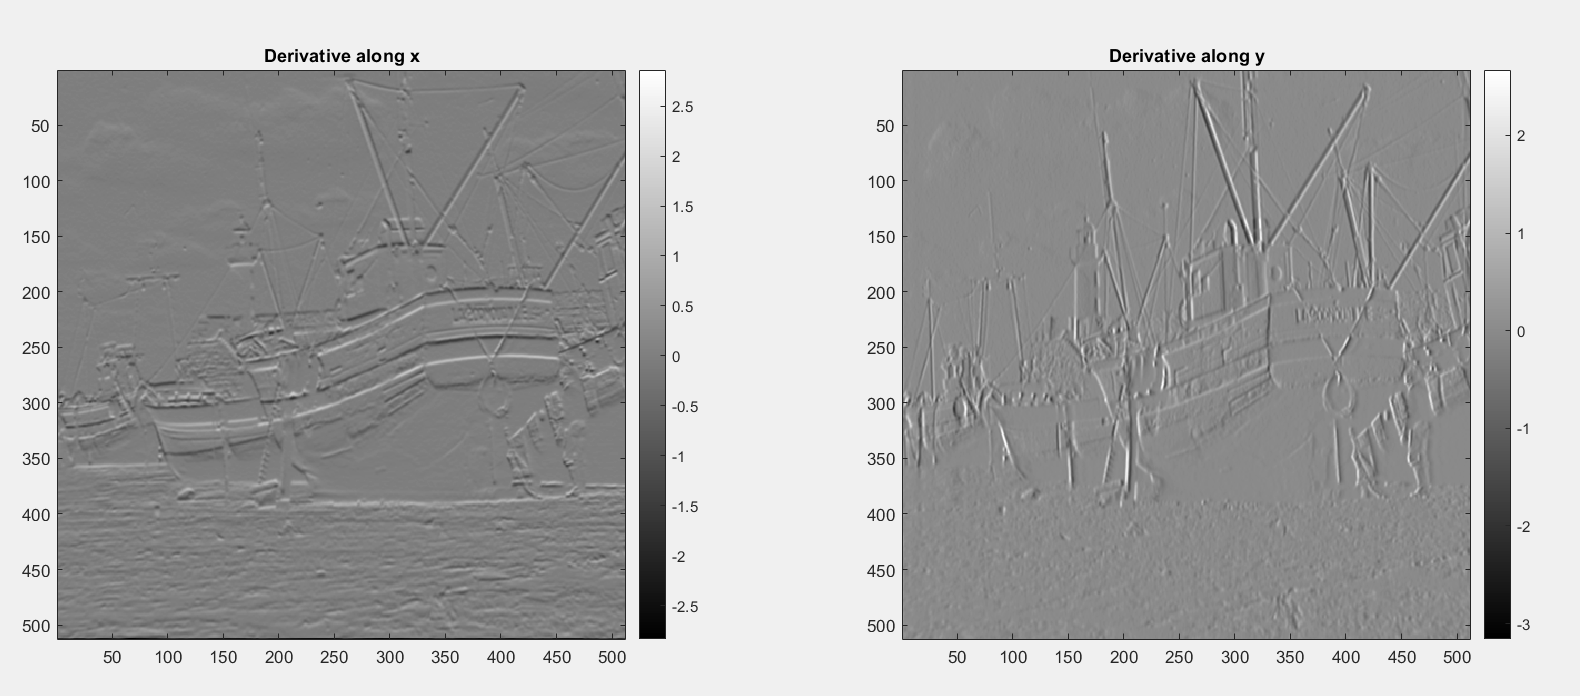
\includegraphics[scale=0.4]{derivative.png}
    \caption{Derivative along X and Y}
  \label{fig:1}
\end{figure}

\begin{figure}[h!]
  \centering
    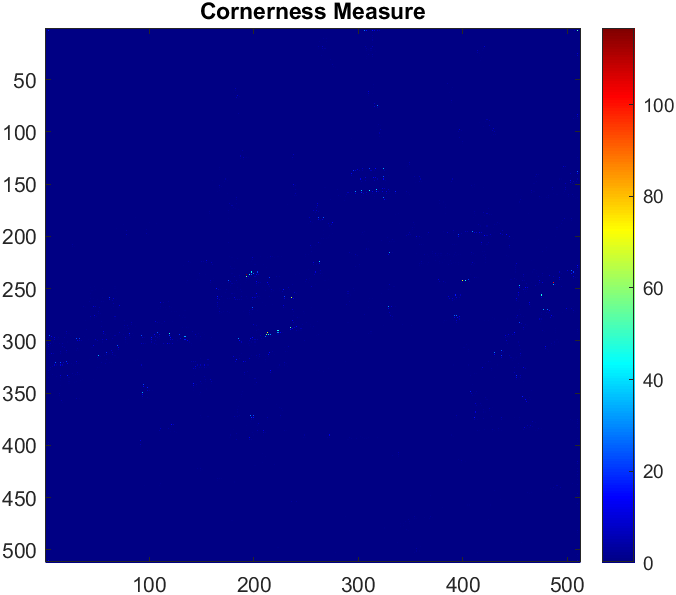
\includegraphics[scale=0.8]{cornerness_measure.png}
    \caption{Cornerness measure}
  \label{fig:2}
\end{figure}

\begin{figure}[h!]
  \centering
    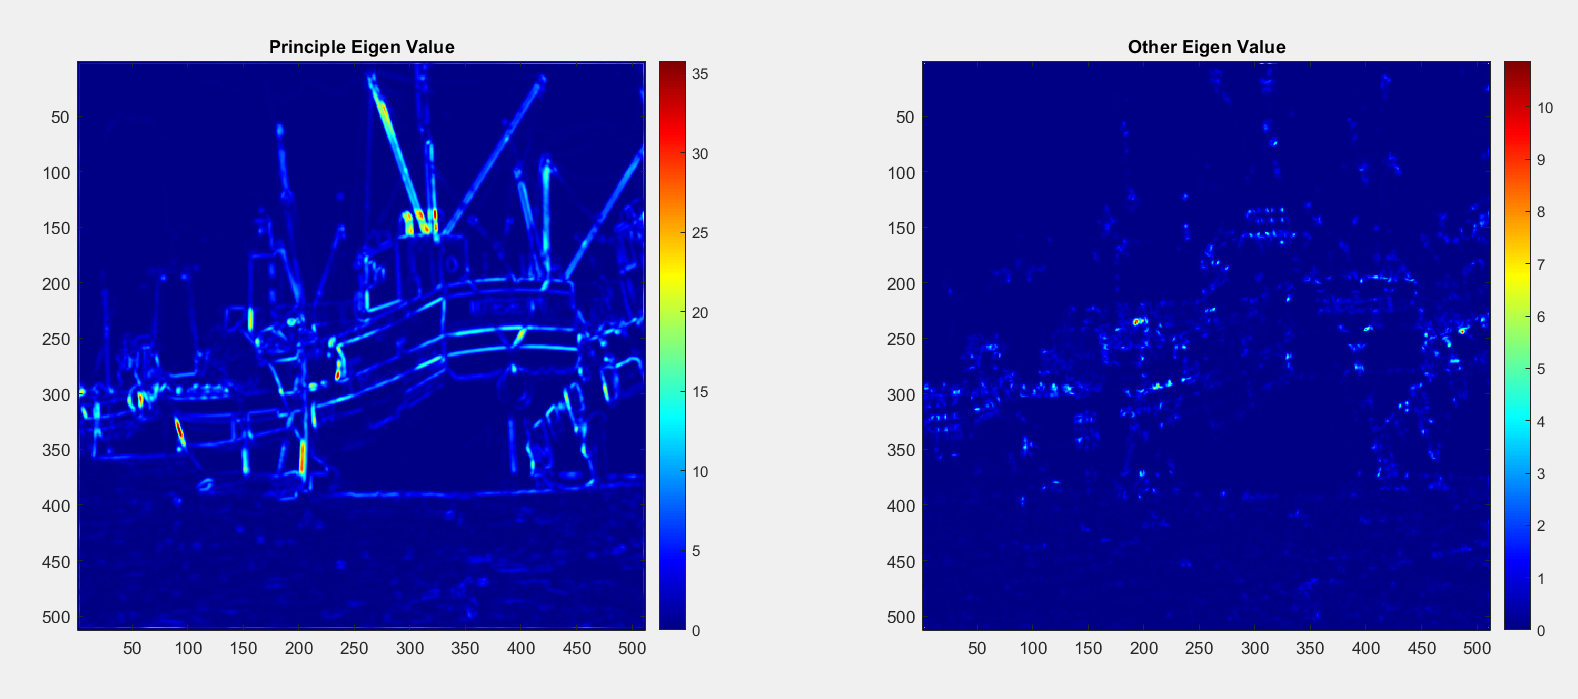
\includegraphics[scale=0.4]{eigen_values.png}
    \caption{Eigen values}
  \label{fig:3}
\end{figure}

\subsection*{Code Usage}
The main file myMainScript.m is divided into 2 parts. 
\begin{itemize}
    \item Firstly we use gaussian filter  to smoothen the image. Then we use sobel filter to get the derivative along X and Y directions. Then we calculate the cornerness measure image using myHarrisCornerDetector.m function.
    \item The second part uses the technique of non-maximal suppression to get the final output.
\end{itemize}
\end{document}
